\documentclass[a4paper ,12pt, onecolumn]{article}
\usepackage[utf8]{inputenc}
\usepackage[spanish]{babel}
\usepackage[hidelinks]{hyperref}
\usepackage{graphicx}
\begin{document}
\title{Anexo desarrollo de hardware}

\author{Rubén Arce}
\date{\today}
\maketitle
\cleardoublepage
\tableofcontents
\cleardoublepage

\section{Introducción}
    Los diseños eléctricos y trazado de las pistas del circuito se han llevado a cabo con Kicad en 
    su versión 5.1.6, se ha empleado este programa debido a que, en primer lugar es de software abierto y
    completamente gratuito y en segundo lugar debido a que corre en linux y es capaz de llevar a cabo 
    cualquier diseño complejo sin problema.
    \paragraph{}
    Todas las PCBs se han llevado a cabo en dos capas con un espesor estándar de 1,6mm y con acabado superficial
    HASH plomo estaño en los primeros prototipos. En la verisión final se empleará acabado ENIG, o de oro 
    electrolítico para mejorar las especificaciones y durabilidad de la misma.
\section{Emisor beacon}
    \subsection{Aspectos a considerar}
        \begin{enumerate}
            \item Bajo consumo
            \item Tamaño reducido
            \item bluetooth
        \end{enumerate}
    \subsection{Circuito eléctrico}
        \subsubsection{Microcontrolador} 
            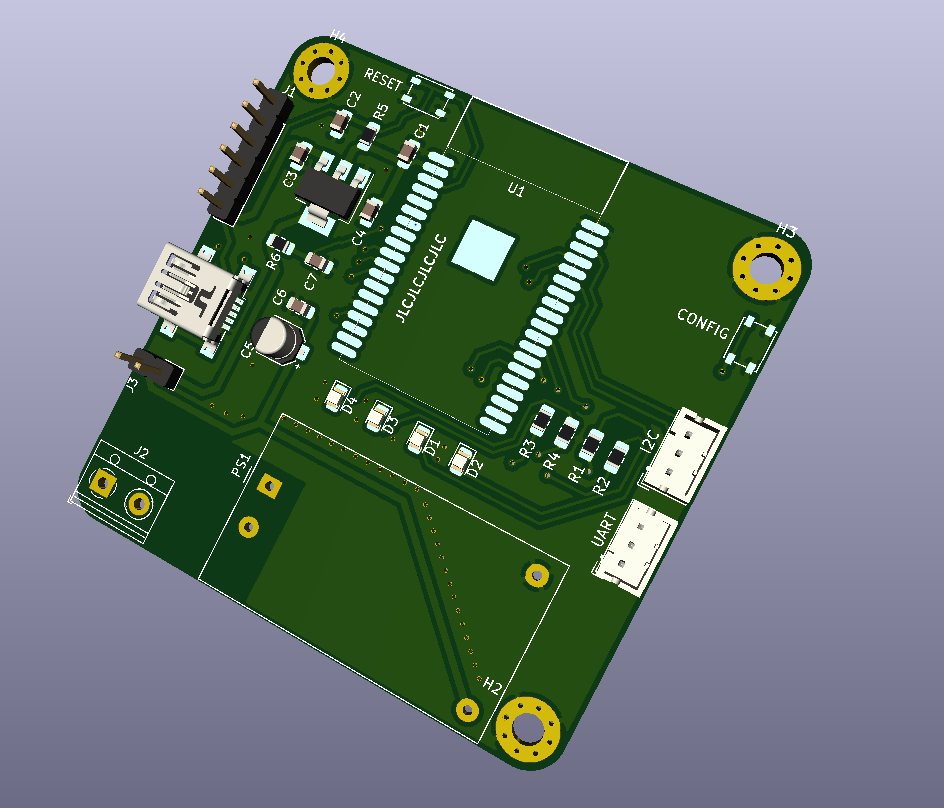
\includegraphics[scale=0.4]{../receiver_1.PNG}
        \subsubsection{Alimentación} 
            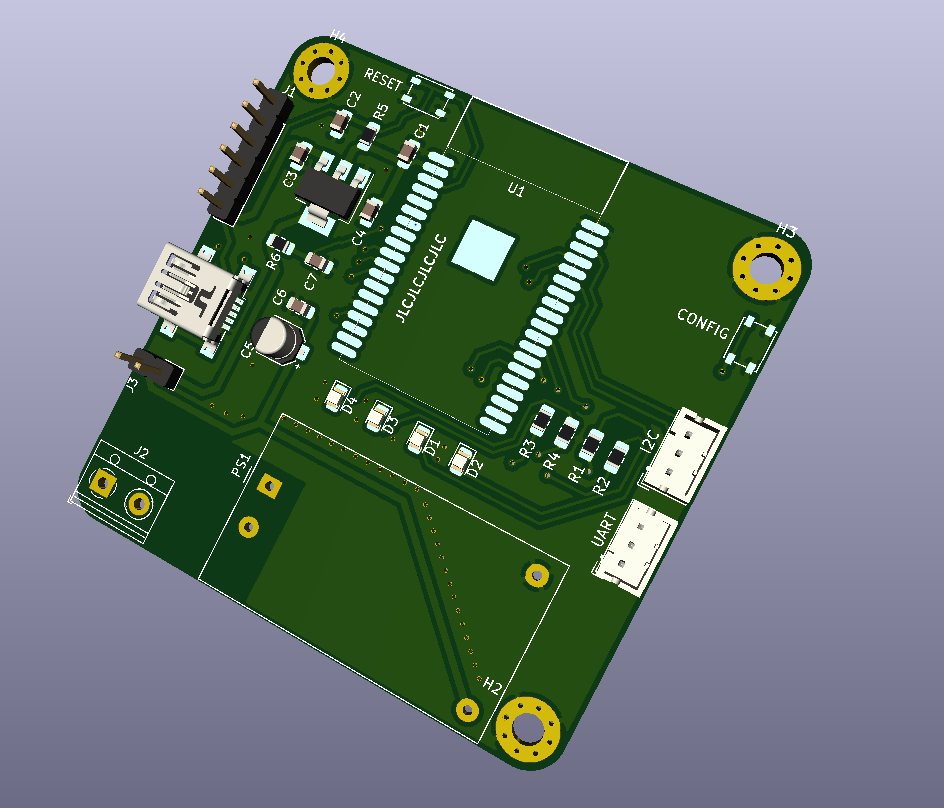
\includegraphics[scale=0.4]{../receiver_1.PNG}
    \subsection{PCB de control}
        \paragraph{}
        Una vez tenidas en cuenta estas especificaciones en el esquema eléctrico 
        se ha llevado a cabo el ruteo de la tarjeta.
        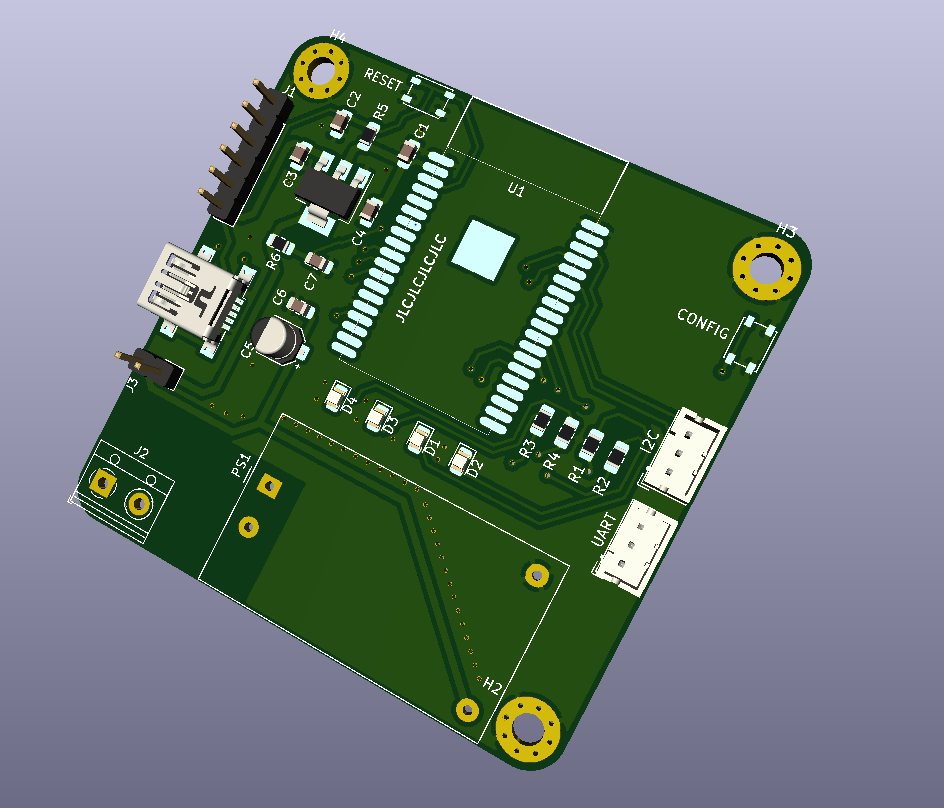
\includegraphics[scale=0.4]{../receiver_1.PNG}
        Vemos que se han llevado a cabo el trazado de pistas con planos de masa para evitar la 
        electricidad estática de las personas no afecte demasiado a la electrónica.
    \subsection{Imágenes renderizado}   
        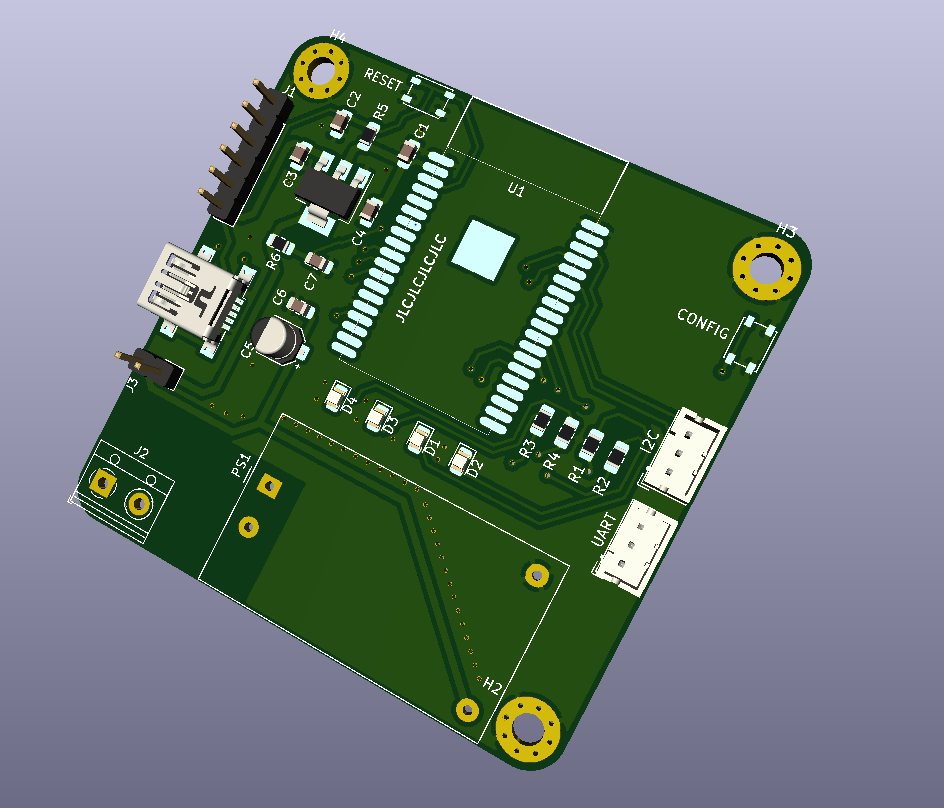
\includegraphics[scale=0.4]{../receiver_1.PNG}
        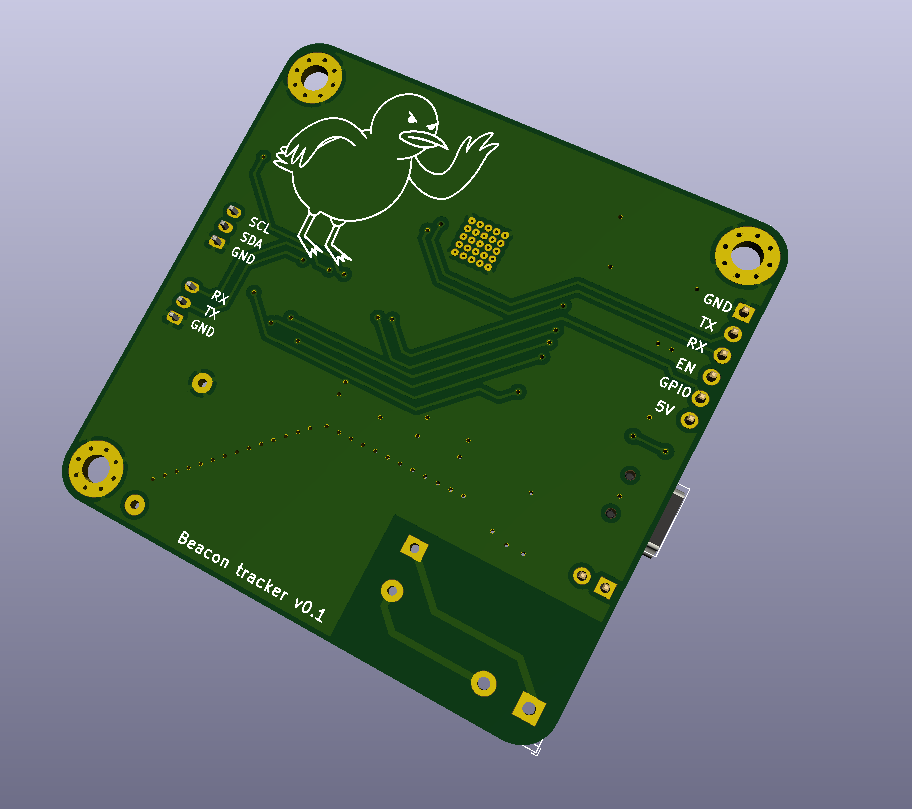
\includegraphics[scale=0.4]{../receiver_2.PNG}
    \subsection{Imágenes reales}

\section{Receptor beacon o gateway}
    \subsection{Aspectos a considerar}
        \begin{enumerate}
            \item Velocidad de procesamiento:
            \item Wifi/bluetooth:
        \end{enumerate}
    \subsection{Circuito eléctrico}
    \subsection{PCB de control}
    \subsection{Imágenes renderizado}
        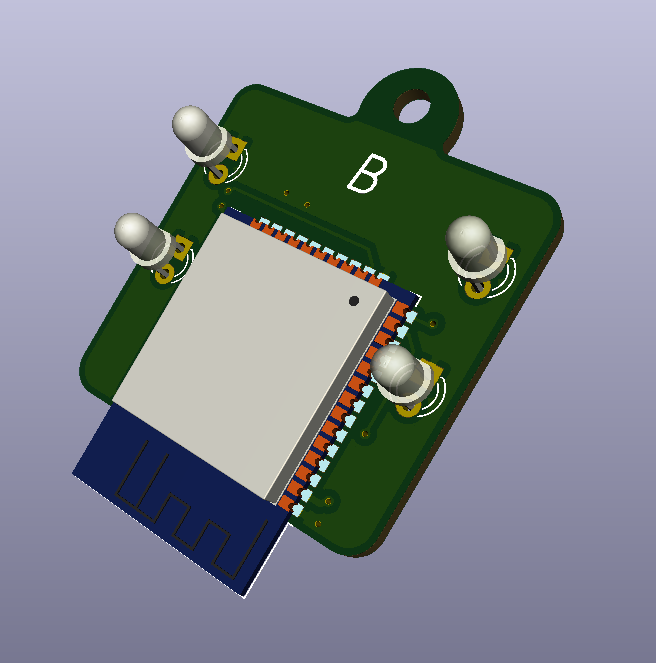
\includegraphics[scale=0.4]{../emiter_1.PNG}
        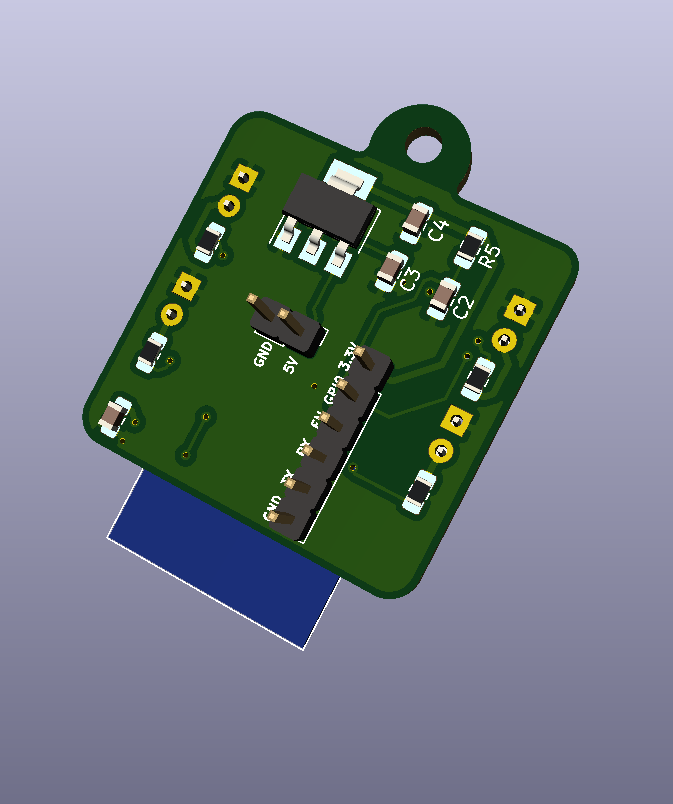
\includegraphics[scale=0.4]{../emiter_2.PNG}
    \subsection{Imágenes reales}

\section{Bibliografía}
https://www.bluetooth.com/
\end{document}